% \setchapterpreamble[u]{\margintoc}
\chapter{Phenomenology of TeV Neutrinos}
\labch{nu_theory}
% \begin{figure}[h]
%     \caption{Measured and predicted neutrino fluxes of neutrinos from various natural sources. Solar neutrinos are neutrinos, while geo-neutrinos and nuclear reactors (terrestrial) are antineutrinos. Other sources produce roughly equal numbers of neutrinos and antineutrinos. Neutrinos from the Big Bang, diffuse supernova neutrinos, and high-energy cosmogenic neutrinos remain undetected. Figure from \cite{KATZ2012651}}
%     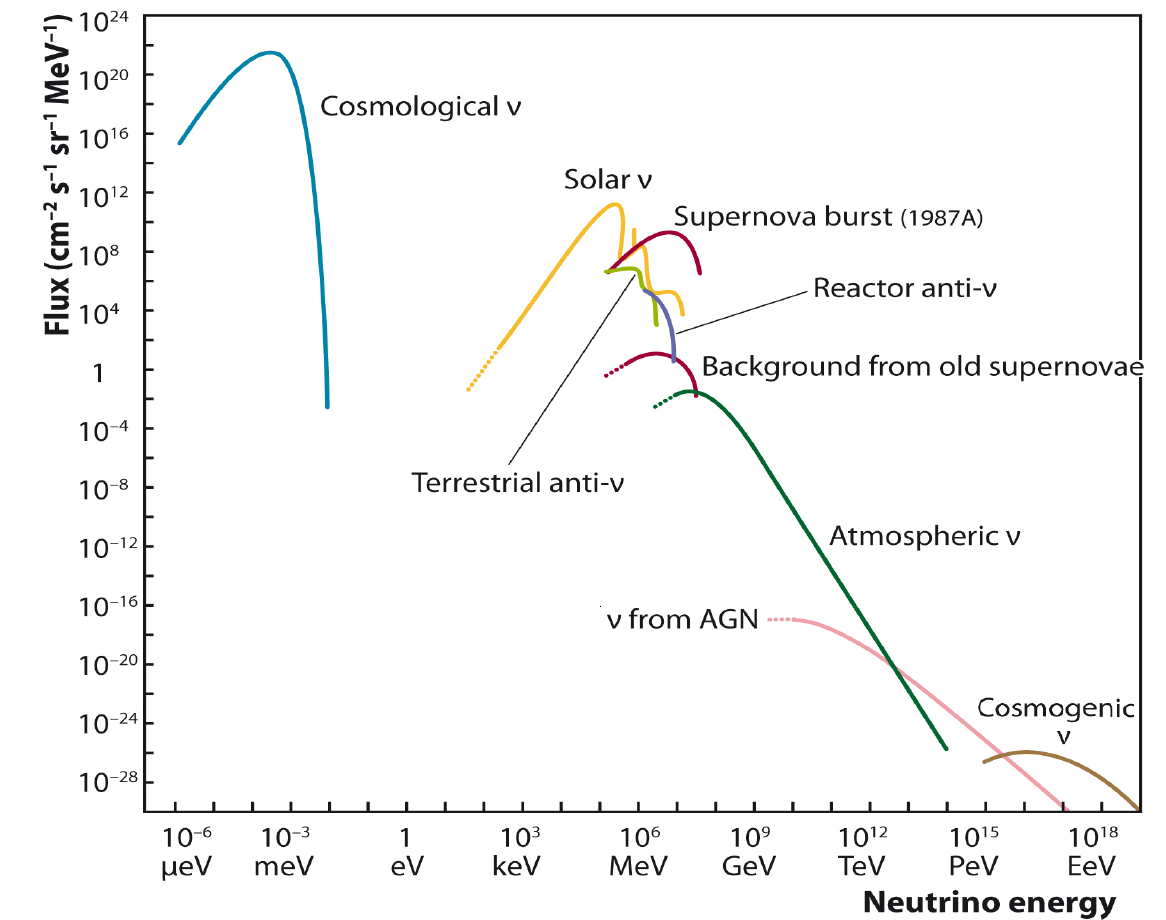
\includegraphics{./figures/nu_phenomenology/all-nu-spectrum-mod.png}
%     \labfig{nu_spectrum}
% \end{figure}
The concept of the neutrino, initially called the "neutron," was first proposed by Pauli in 1930 \sidecite{Pauli} to explain the observed continuous energy spectrum in the beta decay process. Even 60 years after the first direct detection of neutrinos from nuclear reactors by Cowan and Reines \sidecite{nu_discovery}, neutrinos are still the subject of intense experimental investigation, and many of their fundamental properties remain to be measured. This chapter details fundamental properties of Neutrinos in standard model, their interactions and other properties. Last section shall highlight properties and interactions assuming theories \emph{Beyond Standard Model}.
% Neutrinos are produced by various sources across a very large energy range (see \reffig{nu_spectrum}), including particle accelerators, nuclear reactors, and several natural processes. The largest flux of neutrinos comes from nuclear fusion in the Sun \sidecite{Bahcall} and naturally occurring $\beta$-decay on Earth (the so-called \emph{GeoNeutrinos} or \emph{terrestrial neutrinos}) \sidecite{Krauss}. Historically, a similar flux was briefly observed during the supernova SN1987a in the Large Magellanic Cloud, though it only lasted a few seconds \sidecite{SN1987A_superK,SN1987A_Baksan,SN1987A_IMB}. A more constant, but significantly lower, flux is thought to arise from numerous supernovae throughout the universe \sidecite{Vissani}. High-energy neutrinos, above 1 TeV, originate from either atmospheric or astrophysical sources and are of particular interest for the work presented in this thesis. 
\section{Neutrinos in Standard Model}
\label{sec:sm_nu}
Neutrinos are almost massless, electrically neutral fermions with a spin of 1/2. They are categorized into three types: electron, muon, and tau, each associated with a charged lepton counterpart. Neutrinos primarily interact with other particles through the weak nuclear force, and possibly through gravity. In Standard model neutrinos were initially thought to be massless, but when the Homestake experiment measured the flux of solar neutrinos (electron anti-neutrinos) [52], which was one third of what the solar models predicted [53]. 

\subsection{Mass and Oscillations}
\label{sec:nu_mass_osc}

\subsection{Interactions}
\label{sec:nu_interactions}

\subsubsection*{Interaction Cross-Sections}
\label{sec:xsec}

\subsubsection*{Neutrino-Nucleon Deep Inelastic Scattering}
\label{sec:DIS}

\subsubsection*{Glashow Resonance}
\label{sec:glashow}

\subsubsection*{Interaction  Channels}
\label{sec:int_channels}

\subsubsection*{Inelasticty}
\label{sec:inelasticity}


\section{Beyond Standard Model Neutrinos}
\label{sec:bsm}